% 2000 年广东卷第 12 题：圆锥轴截面与 OA
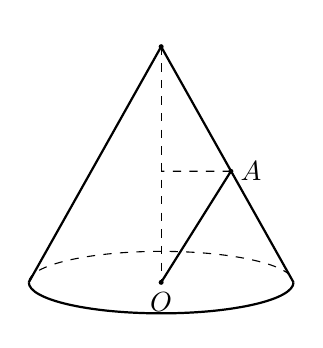
\begin{tikzpicture}[>=stealth, scale=0.82]
  \coordinate (V) at (0,3.65);
  \coordinate (O) at (0,0);
  \coordinate (L) at (-2.05,0);
  \coordinate (R) at (2.05,0);
  \coordinate (A) at (1.08,1.72);
  \draw[thick] (V)--(L) (V)--(R);
  \draw[thick] (L) arc (180:360:2.05 and 0.48);
  \draw[dashed] (L) arc (180:0:2.05 and 0.48);
  \draw[dashed] (V)--(O);
  \draw[thick] (O)--(A);
  \draw[dashed] (A)--(0,1.72);
  \fill (V) circle (1.1pt);
  \fill (O) circle (1.1pt) node[below] {$O$};
  \fill (A) circle (1.1pt) node[right] {$A$};
  \node[above] at (V) { };
\end{tikzpicture}
